%!TEX root=/home/ska124/Dropbox/Thesis/thes-full.tex

%%%%%%%%%%%%%%%%%%%%%%%%%%%%%%%%%%%%%%%%%%%%%%%%%
%
%     Chapter 5
%
%%%%%%%%%%%%%%%%%%%%%%%%%%%%%%%%%%%%%%%%%%%%%%%%

\chapter{Design Choices}
\label{chap:design_choices}


\begin{figure}[ht]
	\small
	\centering
	


% Set the overall layout of the tree
\tikzstyle{level 1}=[level distance=3.5cm, sibling distance=3.5cm]
\tikzstyle{level 2}=[level distance=3.5cm, sibling distance=2cm]

% Define styles for bags and leafs
\tikzstyle{bag} = [text width=4em, text centered]
\tikzstyle{end} = [circle, minimum width=3pt,fill, inner sep=0pt]

% The sloped option gives rotated edge labels. Personally
% I find sloped labels a bit difficult to read. Remove the sloped options
% to get horizontal labels. 
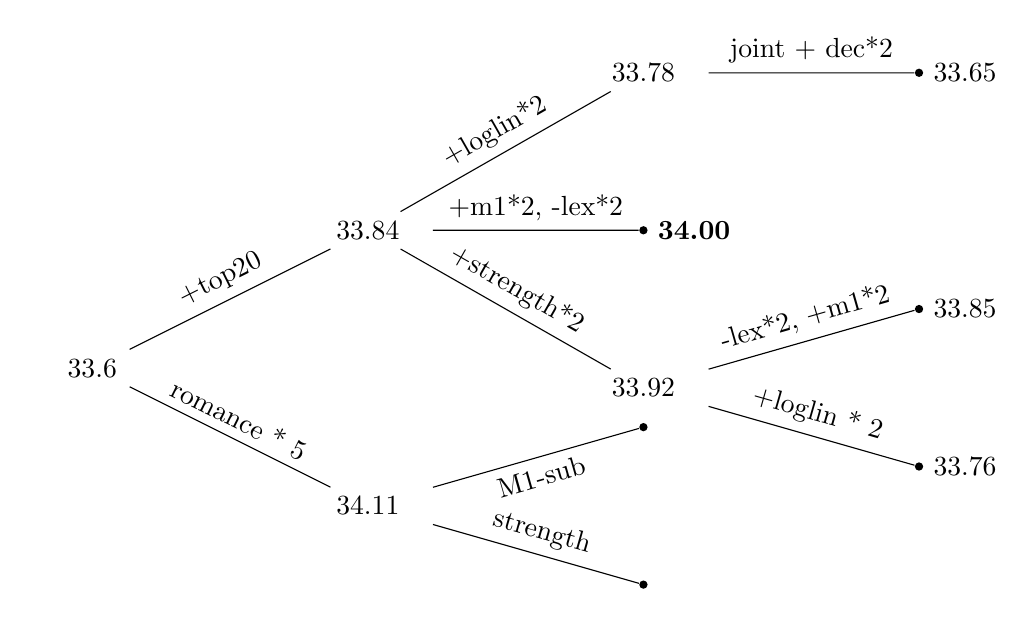
\begin{tikzpicture}[grow=right, sloped][scale=0.4]
\node[bag] {33.6}
	child {
		node[bag] {34.11}
		child {
			node[end, label = left:
			{}] {}
			edge from parent 
			node[above] {strength}
		}
		child {
			node[end, label = left:
			{}] {}
			edge from parent
			node[below] {M1-sub}
		}
		edge from parent
		node[above] {romance * 5}
	}
	child {
		node[bag] {33.84}
	child {
		node[bag] {33.92}
			child {
				node[end, label = right:
				 {33.76}] {}
				edge from parent 
				node[above] {+loglin * 2}
				}
			child {
				node[end, label = right:
				{33.85}] {}
				edge from parent
				node[above] {-lex*2, +m1*2}
			}
		edge from parent
		node[above] {+strength*2}
	}
	child {
		node[end, label = right:
		{\textbf{34.00}}] {}
		edge from parent 
		node[above] {+m1*2, -lex*2}
	}
    child {
        node[bag] {33.78}        
            child {
                node[end, label=right:
                    {33.65}] {}
                edge from parent
                node[above] {joint + dec*2}
            }
            edge from parent
            node[above] {+loglin*2}
    }
    edge from parent
    node[above] {+top20}
    };
   
        
\end{tikzpicture}


	\label{fig:ht_tikz}
	\caption{Diagram of Haiti}
\end{figure}


\begin{figure}[ht]
	\small
	\centering
	


% Set the overall layout of the tree
\tikzstyle{level 1}=[level distance=3.5cm, sibling distance=3.5cm]
\tikzstyle{level 2}=[level distance=3.5cm, sibling distance=2cm]

% Define styles for bags and leafs
\tikzstyle{bag} = [text width=4em, text centered]
\tikzstyle{end} = [circle, minimum width=3pt,fill, inner sep=0pt]

% The sloped option gives rotated edge labels. Personally
% I find sloped labels a bit difficult to read. Remove the sloped options
% to get horizontal labels. 
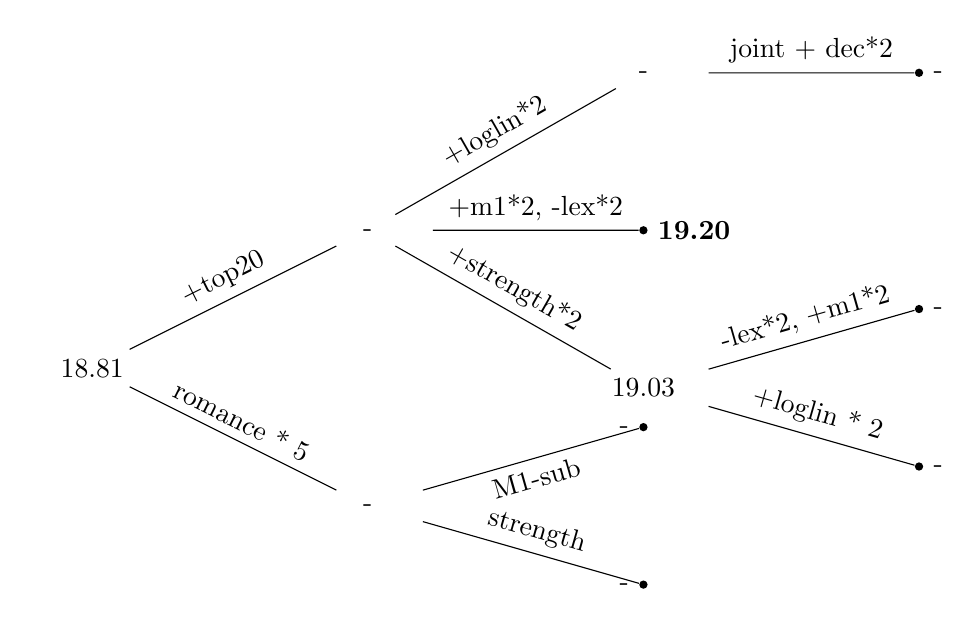
\begin{tikzpicture}[grow=right, sloped][scale=0.4]
\node[bag] {18.81}
	child {
		node[bag] {-}
		child {
			node[end, label = left:
			{-}] {}
			edge from parent 
			node[above] {strength}
		}
		child {
			node[end, label = left:
			{-}] {}
			edge from parent
			node[below] {M1-sub}
		}
		edge from parent
		node[above] {romance * 5}
	}
	child {
		node[bag] {-}
	child {
		node[bag] {19.03}
			child {
				node[end, label = right:
				 {-}] {}
				edge from parent 
				node[above] {+loglin * 2}
				}
			child {
				node[end, label = right:
				{-}] {}
				edge from parent
				node[above] {-lex*2, +m1*2}
			}
		edge from parent
		node[above] {+strength*2}
	}
	child {
		node[end, label = right:
		{\textbf{19.20}}] {}
		edge from parent 
		node[above] {+m1*2, -lex*2}
	}
    child {
        node[bag] {-}        
            child {
                node[end, label=right:
                    {-}] {}
                edge from parent
                node[above] {joint + dec*2}
            }
            edge from parent
            node[above] {+loglin*2}
    }
    edge from parent
    node[above] {+top20}
    };
   
        
\end{tikzpicture}


	\label{fig:mlg_tikz}
	\caption{Malagasy Diagram}
\end{figure}


\begin{figure}[ht]
	\small
	\centering
	


% Set the overall layout of the tree
\tikzstyle{level 1}=[level distance=3.5cm, sibling distance=3.5cm]
\tikzstyle{level 2}=[level distance=3.5cm, sibling distance=2cm]

% Define styles for bags and leafs
\tikzstyle{bag} = [text width=4em, text centered]
\tikzstyle{end} = [circle, minimum width=3pt,fill, inner sep=0pt]

% The sloped option gives rotated edge labels. Personally
% I find sloped labels a bit difficult to read. Remove the sloped options
% to get horizontal labels. 
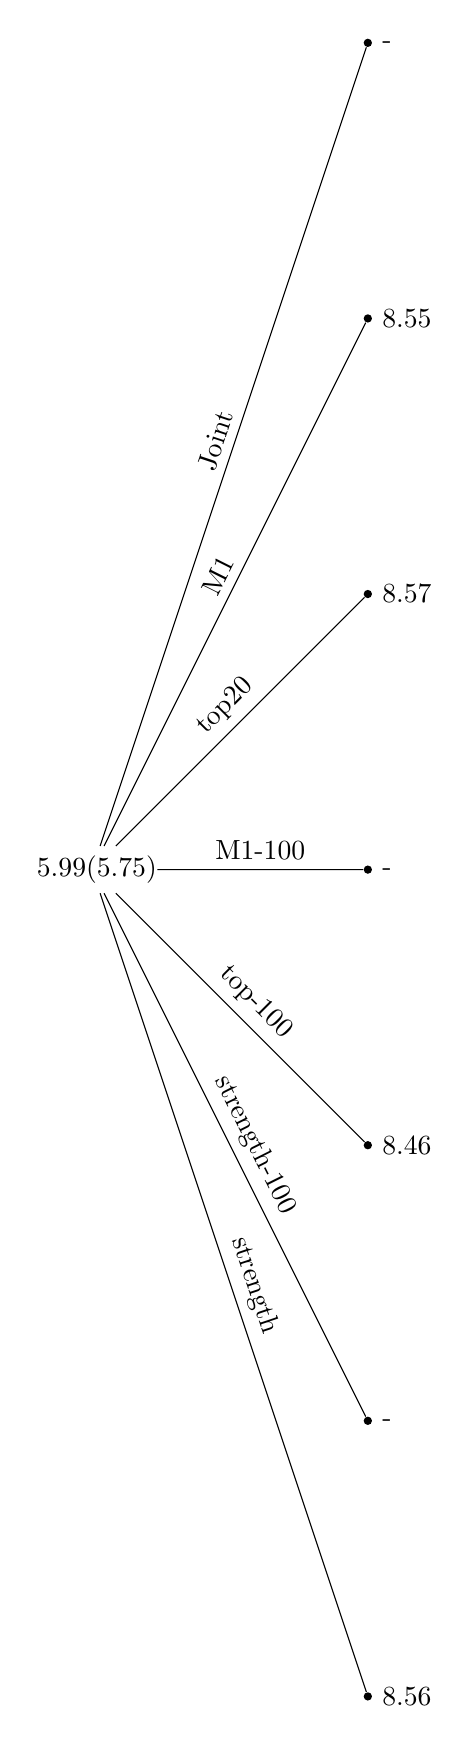
\begin{tikzpicture}[grow=right, sloped][scale=0.2]
\node[bag] {5.99(5.75)}
	child {
		node[end, label = right:
		{8.56}] {}
		edge from parent
		node[above] {strength}
	}
	child {
		node[end, label = right:
		{-}] {}
		edge from parent
		node[above] {strength-100}
	}
	child {
		node[end, label = right:
		{8.46}] {}
		edge from parent
		node[above] {top-100}
	}
	child {
		node[end, label = right:
		{-}] {}
		edge from parent
		node[above] {M1-100}
	}
	child {
		node[end, label = right:
		{8.57}] {}
		edge from parent
		node[above] {top20}
	}
	child {
		node[end, label = right:
		{8.55}] {}
		edge from parent
		node[above] {M1}
	}
	child {
		node[end, label = right:
		{-}] {}
		edge from parent 
		node[above] {Joint}
	};
    
        
\end{tikzpicture}


	\label{fig:mawu_tikz}
	\caption{Mawu Diagram}
\end{figure}

\begin{figure}[ht]
	\small
	\centering
	


% Set the overall layout of the tree
\tikzstyle{level 1}=[level distance=3.5cm, sibling distance=3.5cm]
\tikzstyle{level 2}=[level distance=3.5cm, sibling distance=2cm]

% Define styles for bags and leafs
\tikzstyle{bag} = [text width=4em, text centered]
\tikzstyle{end} = [circle, minimum width=3pt,fill, inner sep=0pt]

% The sloped option gives rotated edge labels. Personally
% I find sloped labels a bit difficult to read. Remove the sloped options
% to get horizontal labels. 
\begin{tikzpicture}[grow=right, sloped][scale=0.4]
\node[bag] {9.96}
	child {
		node[end, label = right:
		{10.76}] {}
		edge from parent
		node[above] {strength}
	}
	child {
		node[end, label = right:
		{10.85}] {}
		edge from parent
		node[above] {strength-100}
	}
	child {
		node[end, label = right:
		{10.76}] {}
		edge from parent
		node[above] {top20}
	}
	child {
		node[end, label = right:
		{11.03}] {}
		edge from parent
		node[above] {top100}
	}
	child {
		node[end, label = right:
		{-}] {}
		edge from parent
		node[above] {m1-100}
	}
	child {
		node[end, label = right:
		{10.57}] {}
		edge from parent
		node[above] {M1}
	}
	child {
		node[end, label = right:
		{-}] {}
		edge from parent 
		node[above] {Joint}
	};
    
        
\end{tikzpicture}


	\label{fig:manin_tikz}
	\caption{Manin Diagram}
\end{figure}

\begin{comment}
\begin{figure}[ht]
	\small
	\centering
	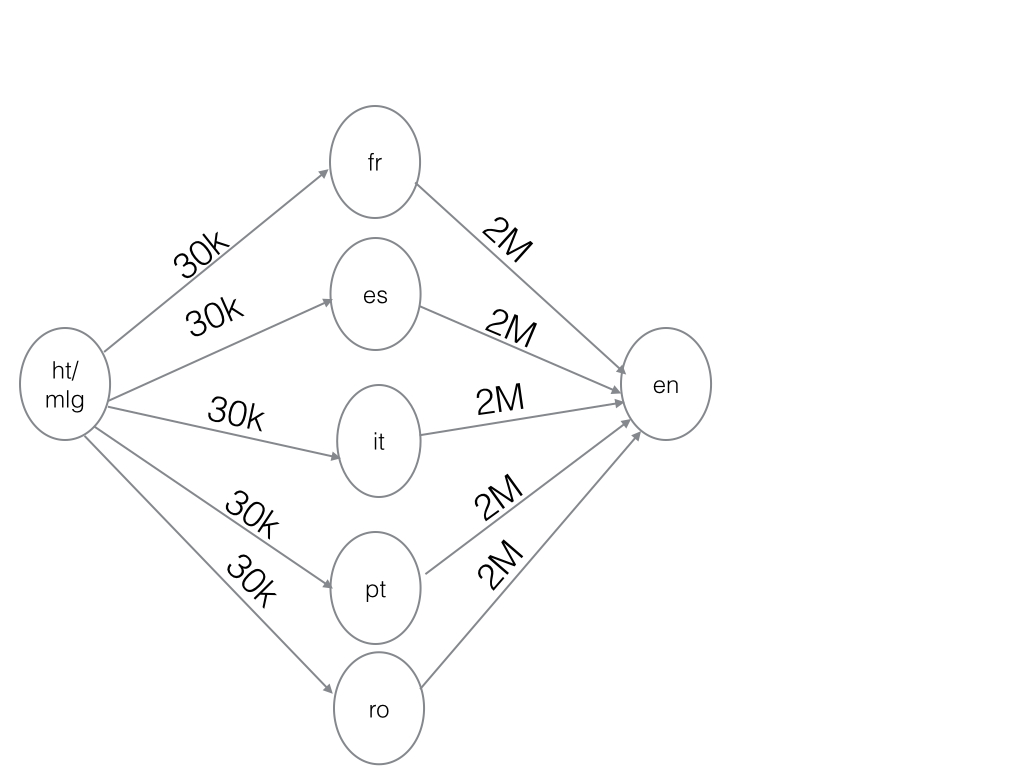
\includegraphics[height=0.5\textheight]{files/Figures/data_multi_pivot.jpg}
	\label{fig:multi_pivots}
	\caption{ht=Haitian-Creole, mlg=Malagasy, en=English, \{fr, it, pt, ro, es\} are the pivot languages}
\end{figure}
\section{Top-n filtering}
\label{sec:topn}

	\subsection{Haitian-Creole}
	\begin{table*}\centering
\small
\begin{tabular}{cllllllclllllll} \toprule
& \multicolumn{6}{c}{$d(cl)$} & \phantom{a} & \multicolumn{6}{c}{$d(r)$} & \phantom{a} \\
\cmidrule{2-7} \cmidrule{9-14} 
& $fr$ & $es$ & $it$ & $pt$ & $ro$ & $\emph{All}$ && $fr$ & $es$ & $it$ & $pt$ & $ro$ & $\emph{All}$  \\
\toprule
$n=20$\\
$$ & 19.84 & 17.21 & 7.29 & - & 9.62 & - && 16.11 & 13.72 & 6.99 & - & 7.98 & -  \\ \toprule
$n=40$ \\
$$ & 19.81 & 17.82 & 7.74 & - & 3.97 & - && 15.92 & 13.80 & 7.36 & - & 3.97 & -  \\ \toprule 
$n=60$ \\
$$ & 20.06 & 17.83 & 6.90 & - & 8.37 & - && 15.96 & 13.76 & 6.98 & - & 7.72 & -  \\ \toprule 
$n=80$ \\
$$ & 19.45 & 16.80 & 4.94 & - & 8.09 & - && 15.36 & 13.46 & 4.91 & - & 7.50 & -  \\
\toprule
$n=100$ \\
$$ & 19.68 & 17.37 & 7.11 & - & - & - && 15.37 & 13.40 & - & 7.01 & - & -  \\
\bottomrule
\end{tabular}
\caption{fr, es, pt, it, ro are the pivot languages, \emph{all} = fr + es + it + pt + ro, d= devtest, cl= clean, r= raw}
\end{table*} 



	\begin{figure}[p]
		\centering
		
\includegraphics[width=\columnwidth]{files/Figures/multi_ht.png}
		\caption{Multiplication Factors: Haitian-Creole}
		\label{fig:multi_ht}
	\end{figure}
	\subsection{Malagasy}


\section{Lexical scores}
\label{sec:lexical_scores}
	\subsection{Haitian-Creole}
	\subsection{Malagasy}

\section{Strength features}
\label{sec:strength_features}
	\subsection{Haitian-Creole}
	\begin{table*}\centering
\small
\begin{tabular}{cllllllclllllll} \toprule
& \multicolumn{6}{c}{$d(cl)$} & \phantom{a} & \multicolumn{6}{c}{$d(r)$} & \phantom{a} \\
\cmidrule{2-7} \cmidrule{9-14} 
& $fr$ & 
$es$ & 
$it$ & 
$pt$ & 
$ro$ & 
$\emph{All}$ && 
$fr$ & 
$es$ & 
$it$ & 
$pt$ & 
$ro$ & 
$\emph{All}$  \\
\toprule
$n=20$\\
$$ & 
19.63 & 
17.50 & 
7.29 & 
7.87 & 
9.90 & 
- && 
15.81 & 
13.70 & 
6.99 & 
7.38 & 
8.23 & 
-  \\ \toprule
$n=40$ \\
$$ & 
20.09 & 
- & 
- & 
2.72 & 
9.60 & 
- && 
16.24 &  
- & 
- & 
2.10 & 
8.12 &
 -  \\ \toprule 
$n=60$ \\
$$ & 
19.57 & 
17.96 & 
7.02 & 
- & 
9.05 & 
- && 
16.07 & 
14.17 & 
7.29 & 
- & 
7.89 & 
-  \\ \toprule 
$n=80$ \\
$$ & 
19.66 & 
15.09 & 
8.15 & 
- & 
- & 
- && 
15.96 & 
12.89 & 
7.89 & 
- & 
- & 
-  \\
\toprule
$n=100$ \\
$$ & 
18.95 & 
13.72 & 
7.40 & 
- & 
9.93 & 
- && 
16.00 & 
11.14 & 
6.91 & 
- & 
8.80 & 
-  \\
\bottomrule
\end{tabular}
\caption{fr, es, pt, it, ro are the pivot languages, \emph{all} = fr + es + it + pt + ro, d= devtest, cl= clean, r= raw}
\end{table*} 


	\subsection{Malagasy}

\section{Phrase scores}
\label{sec:phrase_scores}
	\subsection{Haitian-Creole}
	\subsection{Malagasy}

\section{All-features}
\label{sec:hail_mary}

\section{Multiple pivots}
\label{sec:multiple}

\section{Results}
\label{sec:improved_results}
\end{comment}


